\chapter{Dynamic strip load on 3D elastic halfspace}


% ----------------------------------------------------------------------------------------------
\section{Introduction}
% ----------------------------------------------------------------------------------------------
This document summarises the regression benchmark implemented in
\texttt{test\_strip\_load\_3D.py}. The problem extends the 2D strip load configuration to a
three-dimensional setting by extruding the plane-strain domain over \qty{1}{\meter} in the
out-of-plane direction. The aim is to confirm that the STEM modelling utilities correctly generate
the Kratos input deck, enforce the boundary conditions and recover the stored Linux reference
solution for a rapid surface loading event.


% ----------------------------------------------------------------------------------------------
\section{Model Description}
% ----------------------------------------------------------------------------------------------

% ..............................................................................................
\subsection{Geometry, Mesh and Loading}
% ..............................................................................................
The 3D model represents a \qty{20}{\meter} (x) by \qty{10}{\meter} (y) soil layer extruded to
\qty{1}{\meter} thickness in the z-direction, resulting in a prismatic block. Quadratic
hexahedral-dominant finite elements with a characteristic size of \qty{1}{\meter} are used
throughout the domain, mirroring the mesh settings of the automated test.

A rectangular surface patch bounded by the points $(0,10,0)$, $(1,10,0)$, $(1,10,1)$ and
$(0,10,1)$ carries a uniform downward load with magnitude \qty{1e6}{\newton\per\meter\squared}. The
load is activated instantaneously at $t=0$ and remains constant for the entire analysis:
\begin{equation}
    p(t) =
    \begin{cases}
        0, & t < 0, \\
        \qty{-1000}{\kilo\newton\per\meter\squared}, & t \geq 0.
    \end{cases}
\end{equation}

Boundary conditions emulate the semi-infinite half-space adopted in the python test. The base plane
is fully fixed, while the planes at $x=0$ and $x=20$ operate as rollers by releasing tangential
movement. The front and back faces ($z=0$ and $z=1$) are prevented from moving in the z-direction, so
they mimic symmetry planes and stabilise the thin extrusion.

\begin{figure}
    \centering
    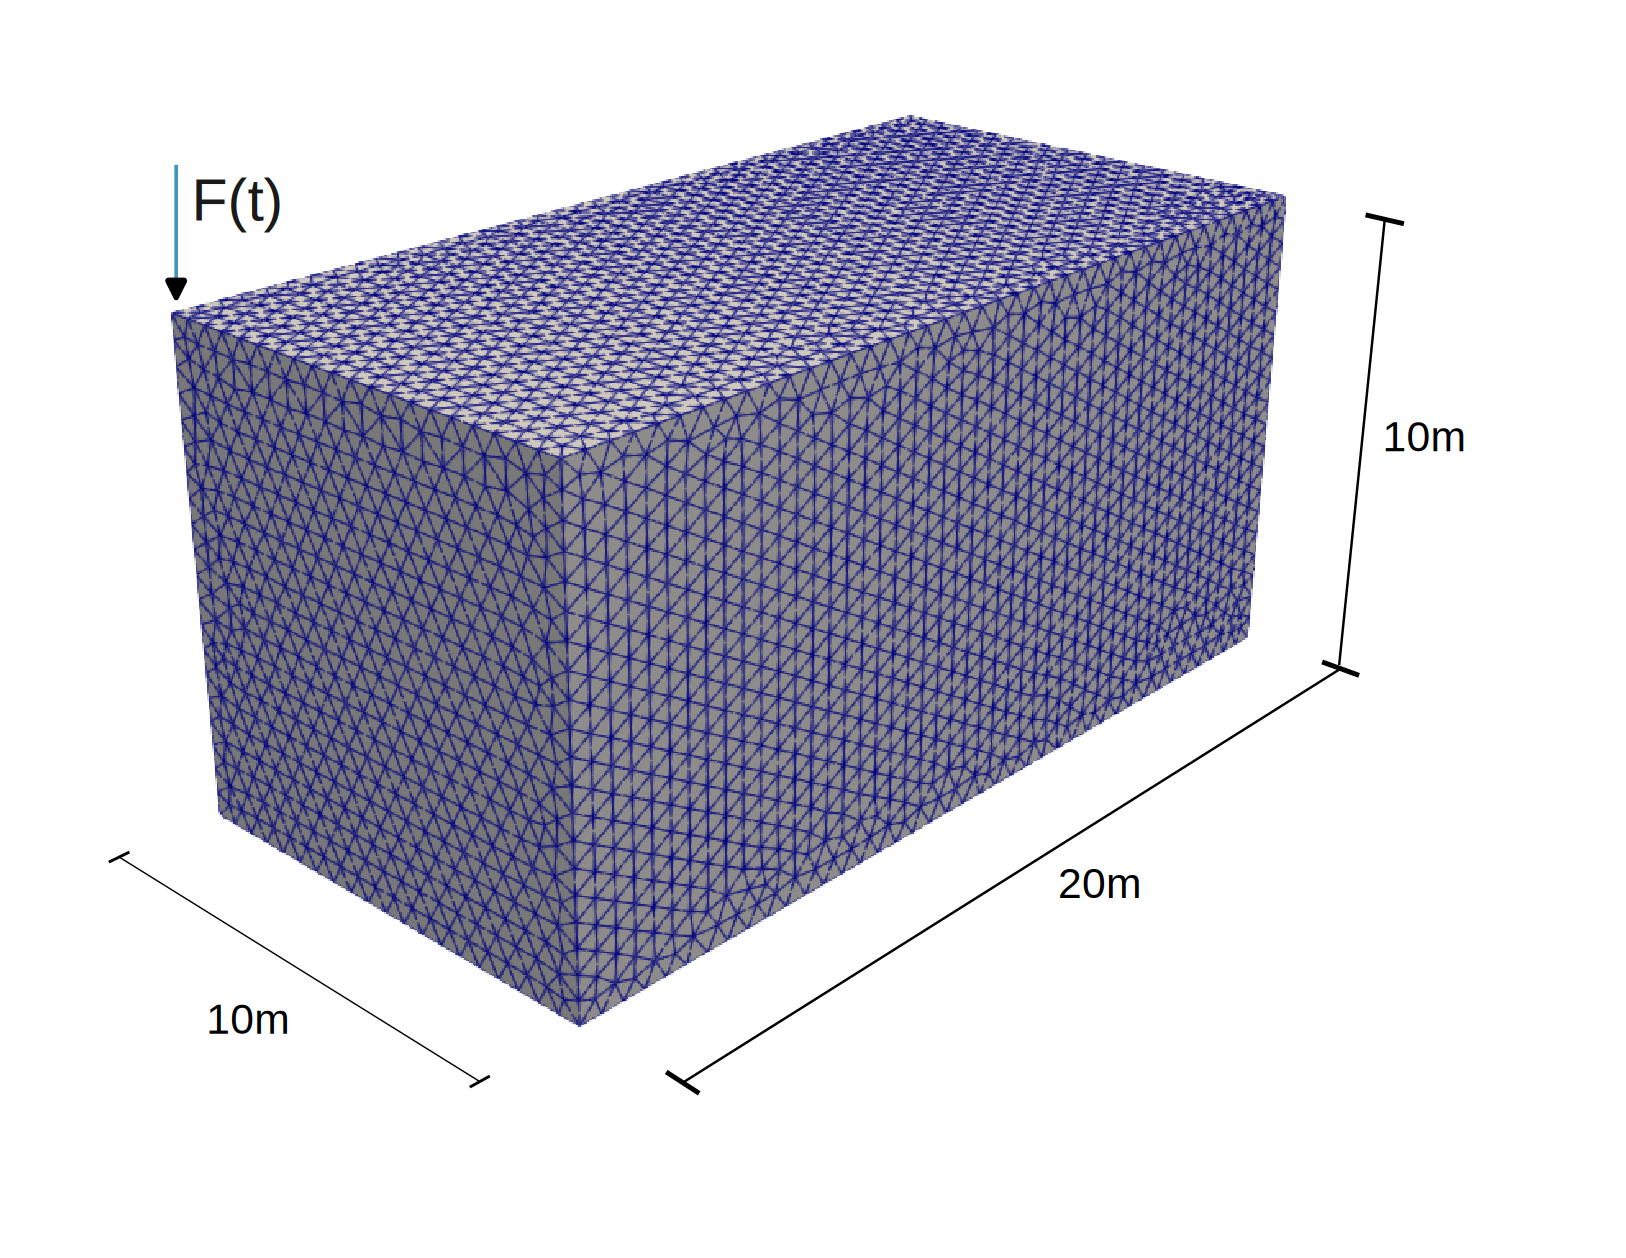
\includegraphics[width=0.75\textwidth]{strip_load_3D/mesh.png}
    \caption{Geometry, mesh and boundary conditions adopted for the 3D strip load benchmark.}
    \label{fig:strip3d_mesh}
\end{figure}

% ..............................................................................................
\subsection{Materials and numerical parameters}
% ..............................................................................................
The soil layer is described by the same drained one-phase, linear elastic material utilised in the
2D counterpart, with parameters:

\begin{itemize}[noitemsep,topsep=0pt,parsep=0pt,partopsep=0pt]
    \item Young's modulus: \qty{30}{\mega\pascal},
    \item Poisson ratio: 0.2,
    \item Density: \qty{2000}{\kilogram\per\meter\cubed}.
\end{itemize}

Time integration uses a constant time step of \qty{0.001}{\second} from $t=0$ to \qty{0.20}{\second}.
Rayleigh damping follows $\alpha = 7.86 \times 10^{-5}$ and $\beta = 0.248$. As in the regression test,
the element matrices are treated as constant and the linear Newton--Raphson strategy couples with the
conjugate gradient solver to obtain the incremental response.


% ----------------------------------------------------------------------------------------------
\section{Results}
% ----------------------------------------------------------------------------------------------

Monitoring points located at $(x,y,z) = (5,10,0)$, $(10,10,0)$ and $(15,10,0)$ track the vertical
velocity response at the surface under the loaded region. Figure~\ref{fig:strip3d_results} contrasts
the STEM output against the stored Linux reference histories. The close match demonstrates that the
3D modelling pipeline, including the extrusion procedure and boundary enforcement, is consistent with
the expected behaviour of the strip load problem.

\begin{figure}[h]
    \centering
    \includegraphics[width=0.8\textwidth]{strip_load_3D/time_history.pdf}
    \caption{Comparison between STEM and reference vertical velocity histories for the three
    monitored nodes.}
    \label{fig:strip3d_results}
\end{figure}
